\section{Developments in \GAP infrastructure: Tools and processes for
  system and package development, quality assurance and release }\label{sec:gap-infra}

As well as developments in the core system and in packages, we have
dedicated considerable effort to improving our infrastructure and processes. 
In this section we describe developments in the technical processes
which support our developers (especially package developers),
connect them to our user community, and aim to 
ensure the robustness and quality of the integrated system, something
essential to its use in demanding large-scale computations.

Associated technical advocacy, training and support
were carried out through \GAP online support channels, as well 
as through development workshops reported in WP2 deliverables D2.2,
D2.11 and D2.15.

\TODO{refer and check w.r.t.
D3.8 \url{https://github.com/OpenDreamKit/OpenDreamKit/blob/master/WP3/D3.8/report-final.pdf}
which has 1,5 pages about GAP CI - but does not discuss many details we provide here}

\subsection{Regression testing}\label{testing}

\emph{Regression testing} %is a software engineering technique which
checks (preferably in an automated way)
that changes and additions to a system do not break functionality that 
worked previously. If a change breaks a test, that is 
a \emph{regression}. In \GAP, regressions may occur
when a change causes an incorrect result, or a crash, or an unwanted error
message; in addition, there may be \emph{performance regressions}
and \emph{memory regressions} where a test becomes slower, or uses
much more memory after a change.

Regression testing has been used by \GAP in one or another form since 
1980s, and by the beginning of the \ODK project, \GAP had established its testing infrastructure
based on a private \href{https://jenkins.io/}{\sf Jenkins} installation
at USTAN, not accessible outside the local network. That was a major limitation,
because sharing test outcomes with other developers and
allowing them to repeat tests in the same environment was cumbersome
and time-consuming with many manual steps.

%\GAP developers came to an understanding 
%that one of the limiting factors (not only for the testing, but for
%the \GAP development in general) was that while \GAP is an open source 
%software, it does not follow an open development model and does not
%have a public source code repository, and just before the start of
%the project established a public source code repository for \GAP
%on GitHub at \url{https://github.com/gap-system/gap}. 

%In the duration of the OpenDreamKit project we, together with other
%contributors to the \GAP project, consolidated \GAP development 
%around GitHub and its tool ecosystem.
%Hosting GAP repository on GitHub and eventual establishing of a number
%of other repositories under the gap-system and gap-packages 
%organizations (\url{https://github.com/gap-system} and 
%\url{https://github.com/gap-packages}), and encouraging package authors 
%to follow the same practices (see \url{https://gap-packages.github.io/})
%to find some further packages that are having public source code 
%repositories elsewhere) allowed us to bring our regression testing
%up to the next level.
%
%\TODO{maybe mention that we can break out onto GitLab if GitHub
%changes in some unacceptable way} 
%

With the widespread adoption of open development models by the
\GAP system and package developers and
maintainers, taking place during \ODK, we have also been able to move
to an open regression testing infrastructure, which has enabled us
to substantially improve \GAP development and testing workflows and
develop a more robust system with less effort. For example,
today, anyone who is interested in checking the
status of the \GAP test suite can visit the public dashboard at
\url{https://github.com/gap-system/gap-distribution/} of which a
snapshot is shown in figure~\ref{fig:gap-core-tests}.
This dashboard shows the status of the core system GAP tests,
which are run for every change made to the repository, as well as
package integration tests described below.

The ``status'' lights are actually active buttons, which lead to the
full test reports, held on the public continuous integration platform
\href{https://travis-ci.org/}{Travis CI}. The the ``code coverage''
lights are also buttons and lead to the public
\href{https://codecov.io/}{Codecov} service, where, if you drill down far
enough, you can access reports showing exactly which lines of code in the kernel
and library have, or have not been tested.

This level of open continuous testing has led to huge imporovements in
the quality of the system, with far fewer bug reports than previously,
and saved enormous effort in integrating releases.

At the heart of the testing of the core \GAP system is achieved by 
the comprehensive test suite. The table below shows its increase
over the period.

% find . -name '*.tst' | wc -l
% find . -name '*.tst' | xargs wc -l
\begin{center}
\begin{tabular}{| l | l | c | c | c |} 
\hline
GAP release & Release date & Number of        & Number of lines & Code coverage \\
            &              & test files       & in test files   &               \\
\hline GAP 4.7.8  & November 2015 (Month 3)   & 69 & 21981 & N/A \\
\hline GAP 4.8.10 & January 2018 (Month 29 )  & 91 & 28586 & N/A \\
\hline GAP 4.9.3  & September 2018 (Month 37) & 564 & 41456 & 69 \% \\
\hline GAP 4.10.2 & June 2019 (Month 46)      & 648 & 53362 & 76 \% \\
\hline GAP 4.11   & November 2019 (planned)   & 707 & 61280 & 84 \% \\
\hline
\end{tabular}
\end{center}

In addition, we also test the correctness of the
over $14,000$ lines in the 1810 examples in our manuals.
%% \comment{1336 mansections containing examples;
%% 1641 (ref) + 169 (tut) = 1810 examples;
%% 13262 (ref) + 940 (tut) = 14202 lines}. 
%% in doc/ref
%Read("makedocreldata.g");
%exsref := ExtractExamples(GAPInfo.ManualDataRef.pathtodoc,
%       GAPInfo.ManualDataRef.main, GAPInfo.ManualDataRef.files, "Chapter");;
%exsref := Filtered( exsref, ch -> Length( ch ) > 0 );;
%Sum(List(exsref,Length));
%Sum(List(exsref, ch -> Sum(List( ch, ex -> Length(Filtered(SplitString(ex[1],"\n"), x -> x<>""))))));
%
%% in doc/tut
%Read("makedocreldata.g");
%exsref := ExtractExamples(GAPInfo.ManualDataTut.pathtodoc,
%       GAPInfo.ManualDataTut.main, GAPInfo.ManualDataTut.files, "Chapter");;
%exsref := Filtered( exsref, ch -> Length( ch ) > 0 );;
%Sum(List(exsref,Length));
%Sum(List(exsref, ch -> Sum(List( ch, ex -> Length(Filtered(SplitString(ex[1],"\n"), x -> x<>""))))));
%%
%% 
% and some further code in the {\tt benchmarks} directory. 
%

We promote a similar testing approach to \GAP package authors and
encourage them to provide their own regression
tests. Many do, adding, in total over a quarter of a million lines of
further tests in the distributed system, which are run when new
versions of packages and/or of the core system are being tested for
integration into a release.

\begin{figure}[!ht]
    \centering
    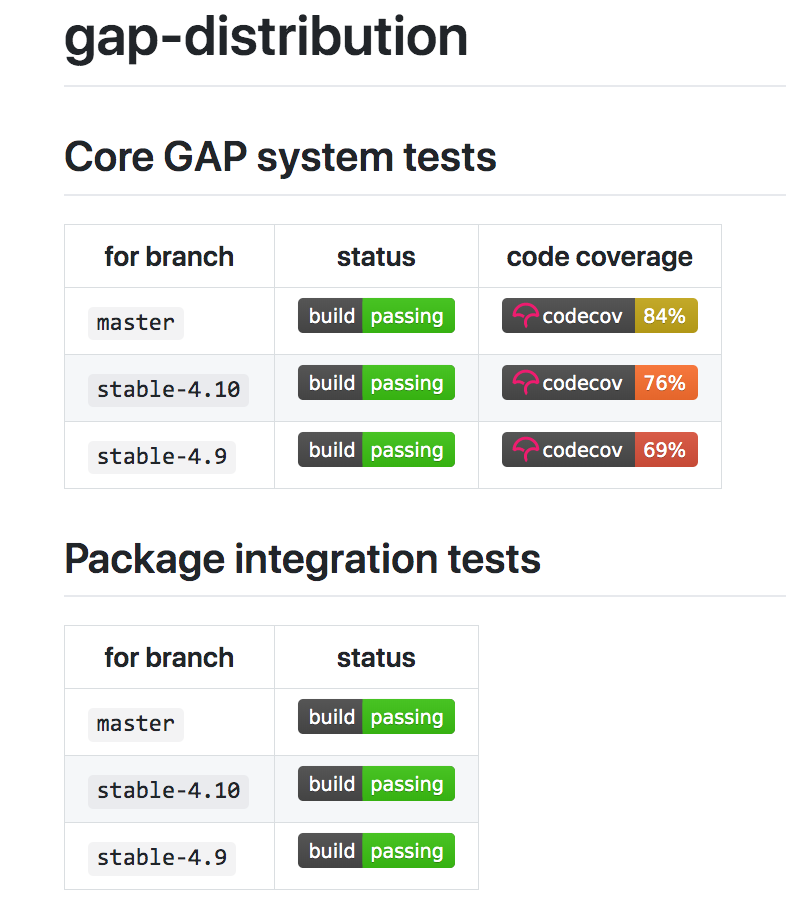
\includegraphics[width=5cm]{images/gap-core-tests}
    \caption{Dashboard with core GAP system and package integration tests}
    \label{fig:gap-core-tests}
\end{figure}

\subsection{Docker containers for testing, using and sharing GAP code}\label{docker}

We continued to maintain and expand the range of Docker containers,
initially reported in D3.1 and then in D3.8. Our main applications of
these containers are:
\begin{itemize}
\item speeding up regression tests by running container-based jobs on Travis CI;
\item sharing reproducible experiments in GAP Jupyter notebooks running on Binder (see Appendix~\ref{sec:repro-gap});
\item as an alternative distributions,
  in particular this helps users who may not have administrator access
  to their systems, to access packages that they cannot run otherwise
  (e.g. due to missing dependencies or incompatibility with the operating system).
\end{itemize}

\begin{figure}[!ht]
    \centering
    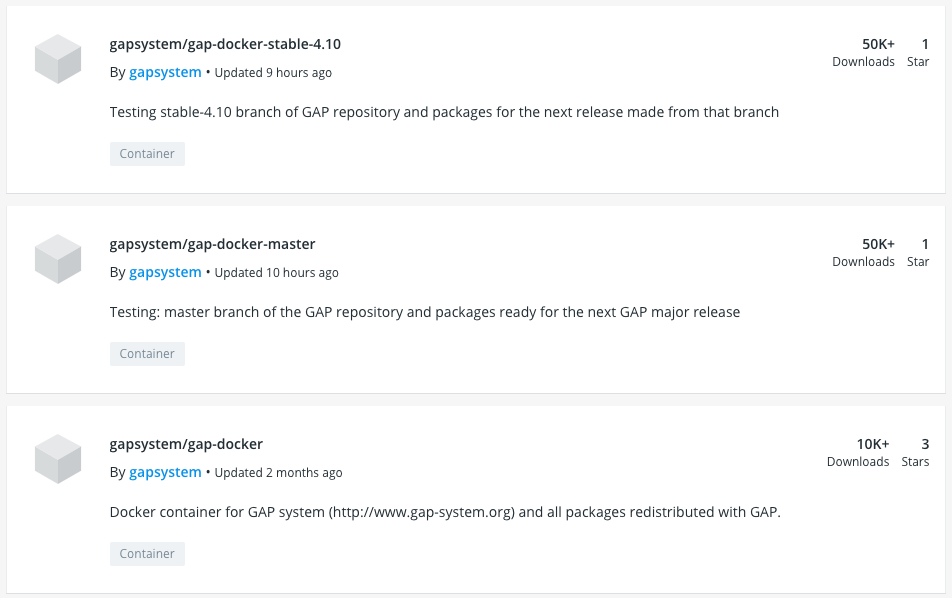
\includegraphics[width=12cm]{images/gap-docker}oif
    \caption{Selected \GAP Docker containers on Docker Hub}
    \label{fig:gap-docker}
\end{figure}

These containers are publicly available on Docker Hub (see Figure~\ref{fig:gap-docker}).
Containers with the development versions of \GAP and packages are updated daily, and have
the largest number of downloads since they are regularly used for testing. An example of
a test using such container could be found under ``Package integration tests'' on
Figure~\ref{fig:gap-core-tests}. Clicking on the ``status'' button leads to the overview displayed
in Figure~\ref{fig:gap-docker-master-testsuite}, from where one could inspect
test output for each of the configurations. 

\begin{figure}[!ht]
    \centering
    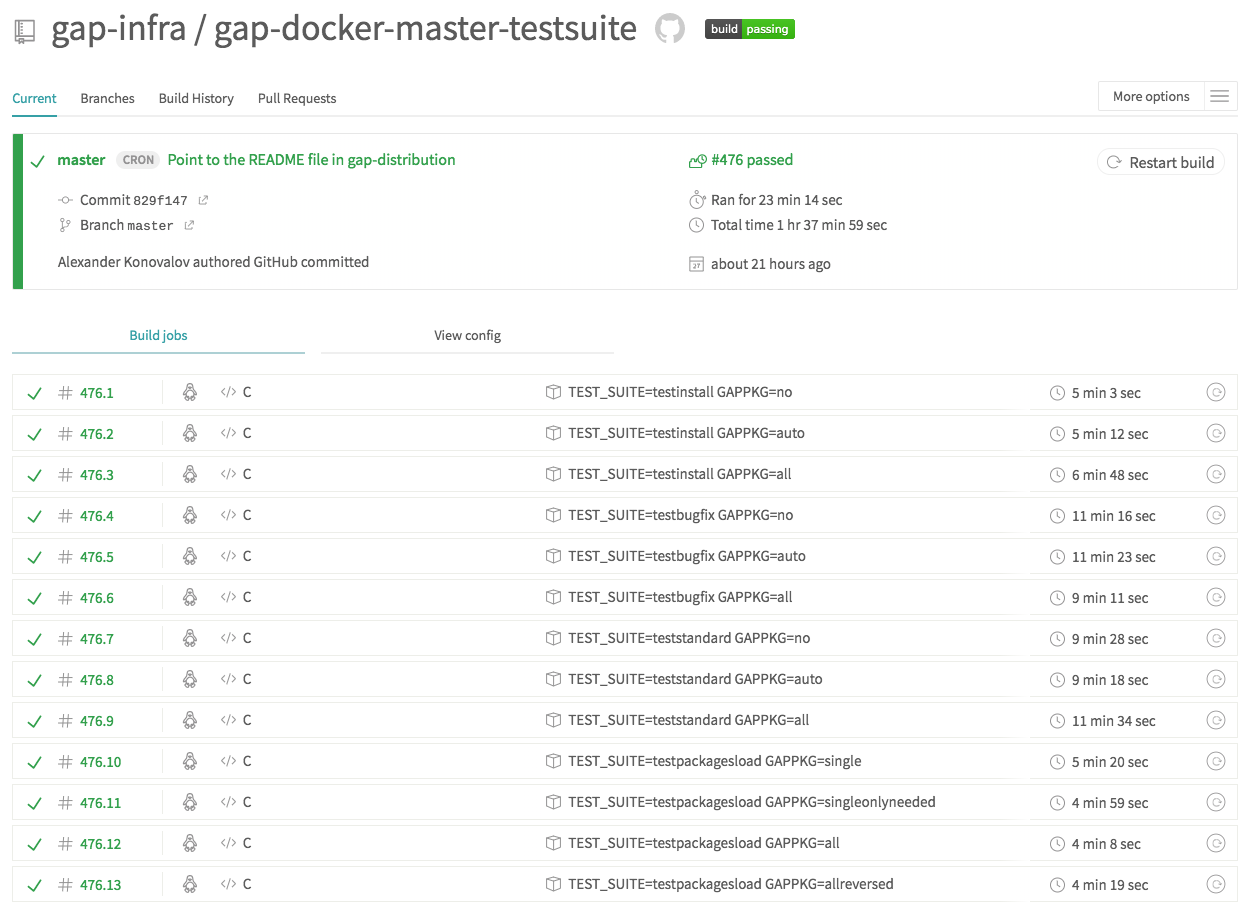
\includegraphics[width=\textwidth]{images/gap-docker-master-testsuite}
    \caption{GAP package integration tests on Travis CI}
    \label{fig:gap-docker-master-testsuite}
\end{figure}

%We made use of \href{https://travis-ci.org/}{Travis CI} and
%\href{https://www.appveyor.com/}{AppVeyor} which are 
%free (for open source projects) continuous integration platforms 
%that can be used to build and test software projects hosted at GitHub.
%\emph{Continuous Integration}, usually abbreviated as {\bf CI} is the process
%automated building and testing for every performed or suggested changes to 
%the source code repository. Using Travis and AppVeyor, one can test changes proposed
%in a pull request \emph{before} they are merged into the main repository.
%At the moment, we use Travis CI for tests on Linux and OS X, and 
%AppVeyor for tests on Windows.

%In addition to that, we started to use \href{https://codecov.io/}{Codecov}
%platform to collect \emph{code coverage} reports for GAP to ensure that our
%regression tests exercise GAP codebase at an acceptable level, and then
%the changes which are submitted via pull request are actually being tested
%by Travis CI. Making these results easily obtainable and publicly available
%had a great effect on the community. Adding new tests to improve code coverage
%is a useful task for new contributors to familiarize themselves with the
%project setup. Making coverage reports available for each pull requests
%facilitates checking code coverage during code review and
%encourages their authors to ensure that their contributions have a good
%quality and their suggested changes are actually being tested. 




%%A crucial role in these developments was played by the enhanced
%%profiling facilities discussed 
%%in Subsection~\ref{gap-4.8}. 
%%GAP~4.8 also introduced the {\tt TestDirectory} function to find
%%(recursively) all {\tt .tst} files from a given directory or a list of 
%%directories and run them using {\tt Test}. Having ability to test
%%changes more efficiently also allowed us to further improve all 
%%tools involved in testing, making their output more informative,
%%and allowing test integration into various automated workflows
%%by a better detection of the test outcomes. 
% the logic seems backwards here. Better test tools let us test better, not v.v.
% What I had in mind was that once we set up the system with the
% state of the testing framework as it was, we were able to "test the testing"
% itself, and improve it - for example, by adding progress indicators,
% report time spent on GC and memory used, etc.




\subsection{Continuous Testing of Package Cross Compatibility Ahead of
\GAP Releases}\label{pkg-update}
For packages redistributed with \GAP, our automatic package update system
checks regularly for new versions on the authors web pages, retrieves them, and then uses them in a
number of checks to ensure that new package releases are compatible with
each other and do not break the functionality of the core \GAP system. The
same process also helps us to check that changes in the core \GAP system
do not break the functionality of the packages redistributed with \GAP.
%% (provided those packages have standard tests that allow us to do that
%% automatically)
This system has dramatically simplified the process of making a \GAP
release or update, for which we need a mutually compatible set of
package versions, also compatible with the new core system. This used
to require extensive negotiation with package authors, and sometimes
took months, even though the number of packages was much smaller. Now
developers have continuous visibility of the functionality and
compatibility of released and upcoming versions of packages and of the
core system, and releases are much faster, delivering new features to
end users without compromising speed of delivery or robustness.

